\documentclass[12pt]{article}

% ------------------------------------------------------------
% Page Layout and Typography
% ------------------------------------------------------------
\usepackage[letterpaper,margin=1in]{geometry}
\usepackage[T1]{fontenc}
\usepackage[utf8]{inputenc}
\usepackage{newtxtext}
\usepackage{newtxmath}
\usepackage{setspace}
\usepackage{indentfirst}
\setstretch{1.15}
\usepackage{microtype}
\usepackage{parskip}
\setlength{\parindent}{0.25in}
\setlength{\parskip}{0.55em}

% ------------------------------------------------------------
% Tables, Figures, Links, and Formatting
% ------------------------------------------------------------
\usepackage{booktabs}
\usepackage{tabularx}
\usepackage{array}
\usepackage{float}
\usepackage{caption}
\usepackage{xcolor}
\usepackage{xurl}
\usepackage[hidelinks]{hyperref}
\usepackage{titlesec}
\usepackage{fancyhdr}
\usepackage{lastpage}
\usepackage{enumitem}
\usepackage{graphicx}

\definecolor{reportblue}{HTML}{173A5E}
\definecolor{lightblue}{HTML}{EEF5FB}
\definecolor{darkgray}{HTML}{333333}

\hypersetup{
    colorlinks=true,
    linkcolor=reportblue,
    urlcolor=reportblue,
    citecolor=reportblue
}
\urlstyle{same}
\sloppy

% ------------------------------------------------------------
% Section Styling
% ------------------------------------------------------------
\titleformat{\section}
  {\normalfont\Large\bfseries\color{reportblue}}
  {\thesection}{0.75em}{}
\titleformat{\subsection}
  {\normalfont\large\bfseries\color{darkgray}}
  {\thesubsection}{0.75em}{}
\titlespacing*{\section}{0pt}{1.35em}{0.65em}
\titlespacing*{\subsection}{0pt}{1em}{0.4em}

% ------------------------------------------------------------
% Header and Footer
% ------------------------------------------------------------
\setlength{\headheight}{15pt}
\pagestyle{fancy}
\fancyhf{}
\fancyhead[L]{Jared Wood}
\fancyhead[C]{Ethical Hacking, RF, and AI}
\fancyhead[R]{\thepage\ of \pageref{LastPage}}
\renewcommand{\headrulewidth}{0.4pt}
\renewcommand{\footrulewidth}{0pt}

% ------------------------------------------------------------
% Custom Boxes
% ------------------------------------------------------------
\newcommand{\reportnote}[1]{%
\begin{center}
\fcolorbox{reportblue}{lightblue}{%
\begin{minipage}{0.93\linewidth}
#1
\end{minipage}}
\end{center}}

% ------------------------------------------------------------
% Title Information
% ------------------------------------------------------------
\title{\vspace{-0.75in}\textbf{Ethical Hacking, Radio Frequency Signals, and Artificial Intelligence}}
\author{Jared Wood}
\date{\today}

\begin{document}

\begin{titlepage}
    \centering
    \vspace*{1.1in}
    {\Huge\bfseries Ethical Hacking, Radio Frequency Signals, and Artificial Intelligence\par}
    \vspace{0.3in}
    {\Large Final Project Report\par}
    \vspace{0.8in}
    {\large Jared Wood\par}
    \vspace{0.15in}
    {\large Ethical Hacking, RF, and AI\par}
    \vfill
    {\large \today\par}
\end{titlepage}

\pagenumbering{roman}
\tableofcontents
\newpage
\pagenumbering{arabic}

\section*{Abstract}
\addcontentsline{toc}{section}{Abstract}

The five layers of ethical hacking as they relate to radio frequency (RF) signals are similar in concept, but the methodology differs. Routinely used applications such as Netcat and Metasploit interact with information that is already inside infrastructure, while RF signals require heavier applications of mathematics, similar to the workflow of a signal intelligence (SIGINT) analyst attempting to understand transmitted signals. Code and artificial intelligence are useful in this setting because they can automate mathematical computation and expedite portions of an otherwise manual SIGINT-style pipeline for predicting signal modulation.

To satisfy the data requirements for model training, DeepSig's RADIOML 2018.01A dataset was downloaded and used for model training and later feature engineering. Three Random Forest Classifiers were created, and the results strongly demonstrated that signal representation and data quality matter significantly more than simply having more data. A reduced highest-SNR dataset of 24,000 signals was used, and the best model was the all-feature-engineered Random Forest with 72.17\% accuracy and 0.9780 weighted ROC-AUC. A simulation was also created to emphasize text modulation and encryption, as well as audio using bit-string manipulation. Overall, the project indicates that AI models have potential for streamlining signal modulation detection, but more exploration is required with noisier signals, encryption, signal timing, and frequency hopping.

\newpage

\section{Introduction}

Communication is vital to survival and is demonstrated throughout the world, from plants and animals to human beings. Regardless of the source, communication is fundamentally rooted in signals and wavelengths. In technology, many communications occur at high frequencies that are inaudible to humans. Just as speech is interpretable to people who understand a language, and slang or code is interpretable to individuals ``in the know,'' inaudible technical signals require the correct interpretation of modulation and, when present, encryption.

In ethical hacking, the general process is described in 5 phases where each phase logically follows the previous one. From lowest to highest, these phases include reconnaissance, scanning, enumeration, maintaining access, and covering tracks. Much of this pipeline interacts with data or information that already exists inside infrastructure such as databases, servers, and web applications.

RF signal analysis is similar in concept but differs in methodology. RF signals are typically data in transit, and they do not inherently track who is listening to them. In the same procedural spirit as ethical hacking, RF signal analysis can be described with adjacent phases: reconnaissance, frequency capture, modulation detection, encryption handling, and deciphered data. This version does not focus on covering tracks; instead, it focuses on being in the correct signal space and using the correct encryption key, when applicable, to receive and interpret transmitted information.

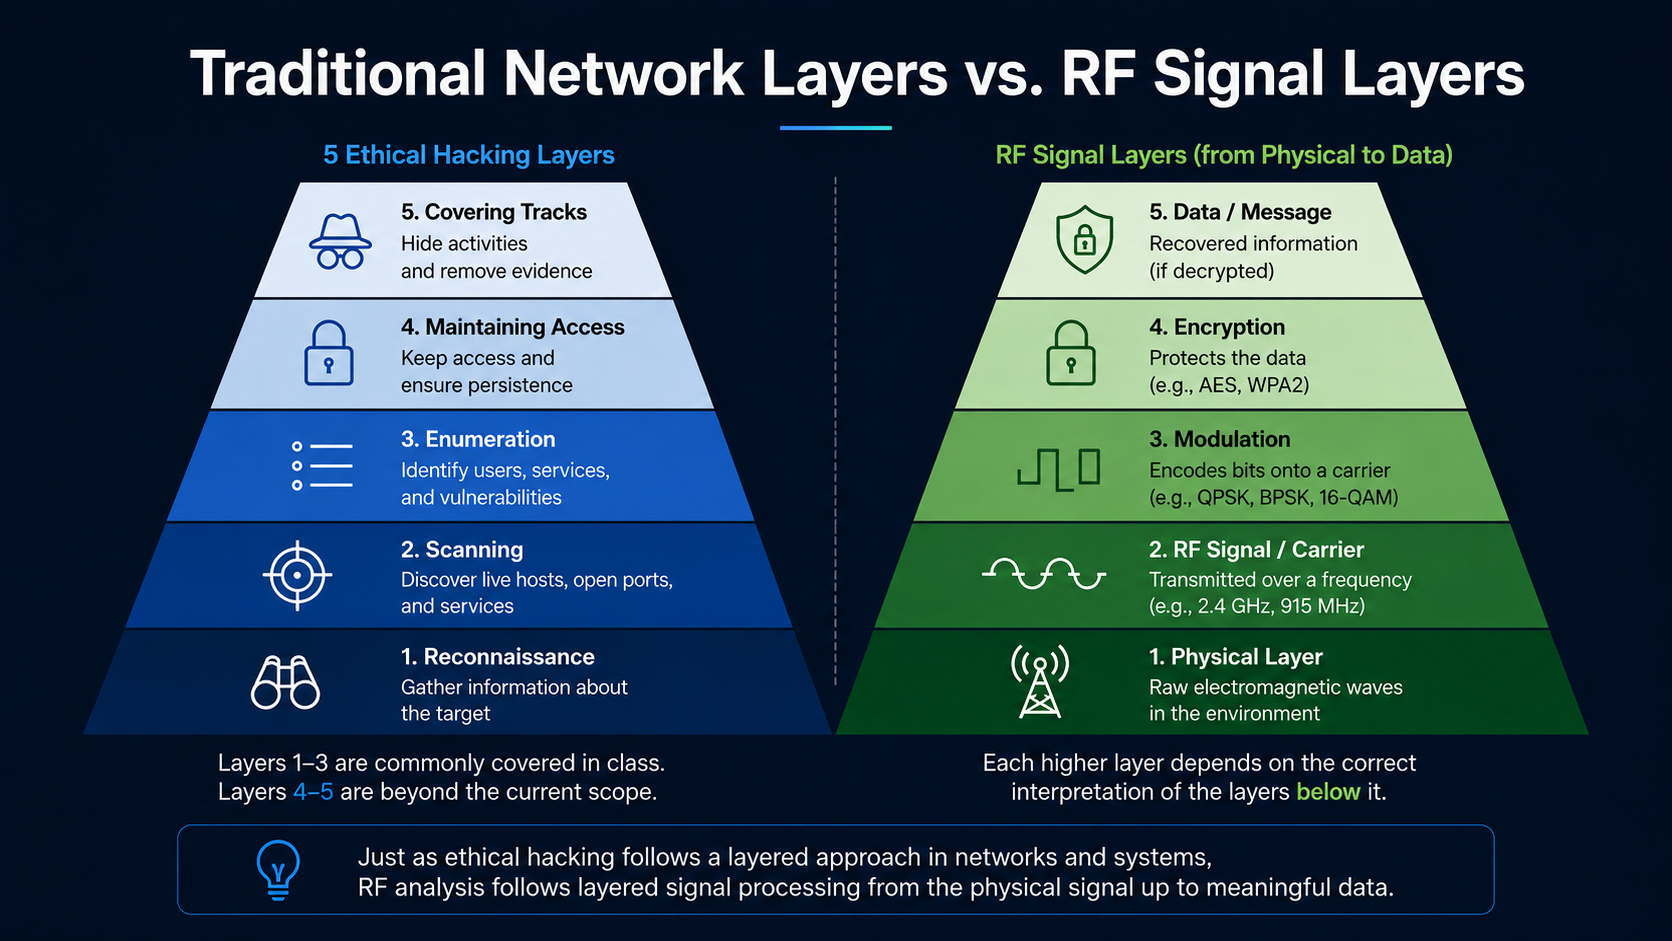
\includegraphics[scale=0.25]{../../KeyImages/layers.png}

\reportnote{\textbf{Project Objective.} This project asks whether an AI model can accurately and reliably take an unknown real-time or recorded signal and successfully support the process of deciphering the information transmitted across the signal. The project ultimately answers this question partially: the model can classify modulation type from recorded I/Q data, but it does not fully decipher unknown real-time RF signals end-to-end.}

\section{Methods}

The primary objective required a data science pipeline: acquiring a reliable dataset, preparing and exploring the dataset, determining an AI model, selecting performance metrics, applying feature engineering and selection, and building a baseline for comparison.

\subsection{Dataset Acquisition and Reduction}

Acquiring a suitable dataset took substantial time because of my limited exposure to signals - since I myself am not a signals subject-matter-expert (SME), but much of my understanding is through these individuals - and because many available datasets either had reading issues or lacked the information needed for a full data science pipeline. Eventually, DeepSig's RADIOML 2018.01A dataset was selected. The dataset contained 2,555,904 signals uniformly distributed over 24 modulation types [5].

The dataset was already very clean and consisted of recorded I/Q values for each signal. Each example had two arrays of 1,024 timestamps: one array representing the in-phase component (I), and the other representing the quadrature component (Q). Each signal was also tagged with a signal-to-noise ratio (SNR) value in the range $[-20, 30]$, where lower SNR values represent noisier captures and higher SNR values represent clearer captures.

For this proof-of-concept and the limitations of my laptop, the dataset was reduced to only the cleanest possible signals, where SNR = 30. I also selected 1,000 signals from each of the 24 modulation types, resulting in a reduced dataset of 24,000 total signals.

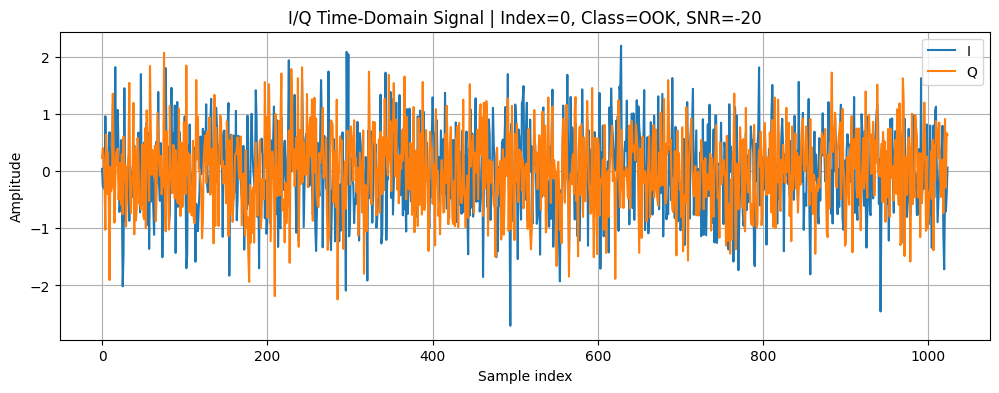
\includegraphics[scale=0.45]{../../KeyImages/ook-20.png}

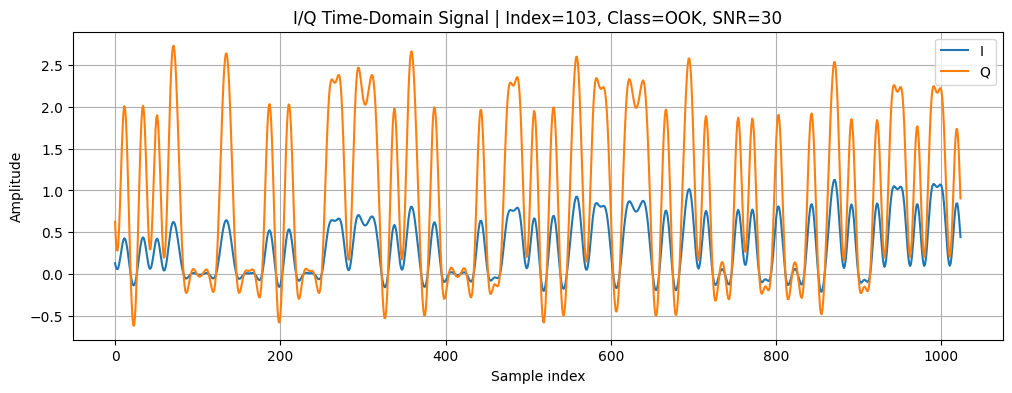
\includegraphics[scale=0.45]{../../KeyImages/ook30.png}

\subsection{Data Preparation and Exploration}

Because the original dataset was clean, structured, and simple, the reduced dataset was also clean, structured, and simple. This allowed me to avoid extensive data cleaning and place more project time on signal representation, model training, feature engineering, and interpretation. This does not mean the data science portion was trivial; instead, it means the project effort was shifted away from cleaning inconsistent records and toward understanding how signal representation affects model performance.

\subsection{Model Selection}

A Random Forest Classifier (RFC) was selected because its methodology is easier to understand, it is lightweight compared to a neural network, and it can reduce the risk of overfitting by combining multiple decision trees [12]. A Random Forest can be understood as a voting system. Each decision tree acts like an individual voter that makes a prediction based on its own view of the data. Once all trees vote, the class with the most votes becomes the model's final prediction. In this project, each tree voted on one of the 24 modulation types for each signal.

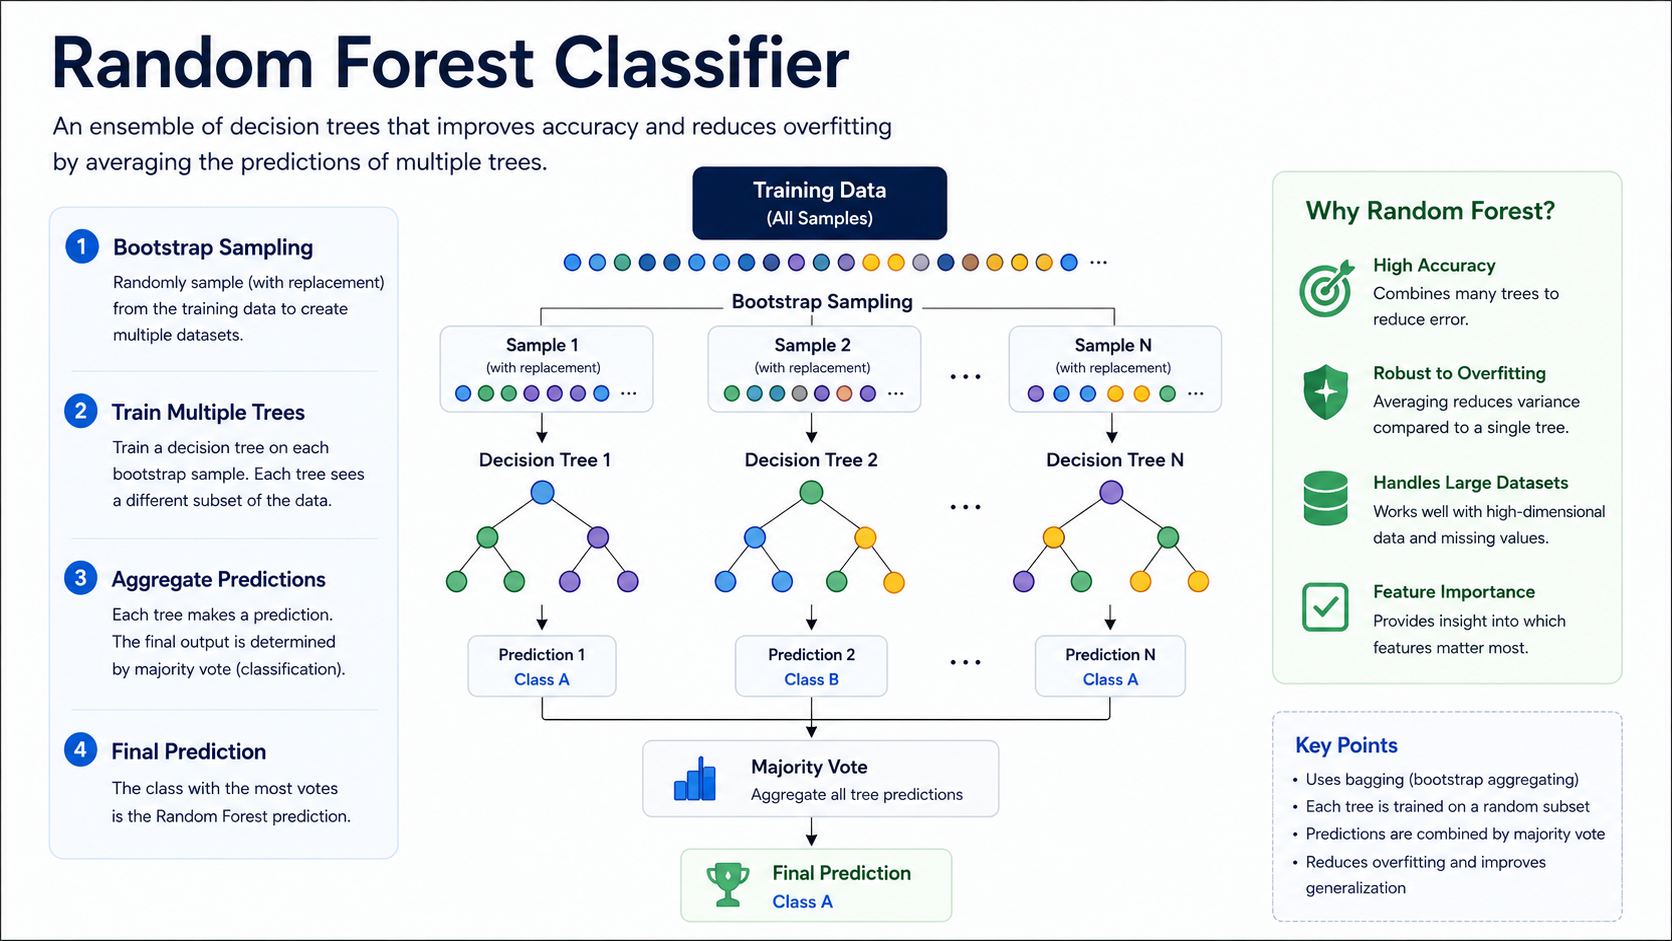
\includegraphics[scale=0.25]{../../KeyImages/rfc.png}

\subsection{Performance Metrics}

I initially chose ROC-AUC to determine whether the trained model predicted better or worse than random guessing across signals. Later, accuracy became the more useful metric because the engineered models had very similar ROC-AUC scores, while accuracy more directly answered the project question: whether the modulation type was correctly predicted. To further reduce the chance of misleading results, the dataset was split into folds for cross-validation, and GridSearchCV was used across a small selection of hyperparameters to tune each respective model.

\subsection{Feature Engineering}

The feature engineering step was strongly rooted in a SIGINT analyst-style pipeline for taking an unknown signal and determining the modulation type. Much of this process involves mathematical transformations that describe the signal from different perspectives, including I/Q statistics, magnitude, power, phase, frequency behavior, Fast Fourier Transform (FFT) features, spectral features, and constellation structure [1], [4], [6], [7].

Because these transformations are established in signal analysis, it was possible to translate the mathematical concepts into code functions. These functions produced engineered features that, in theory, represented similar kinds of information a signal analyst might use to identify modulation type.

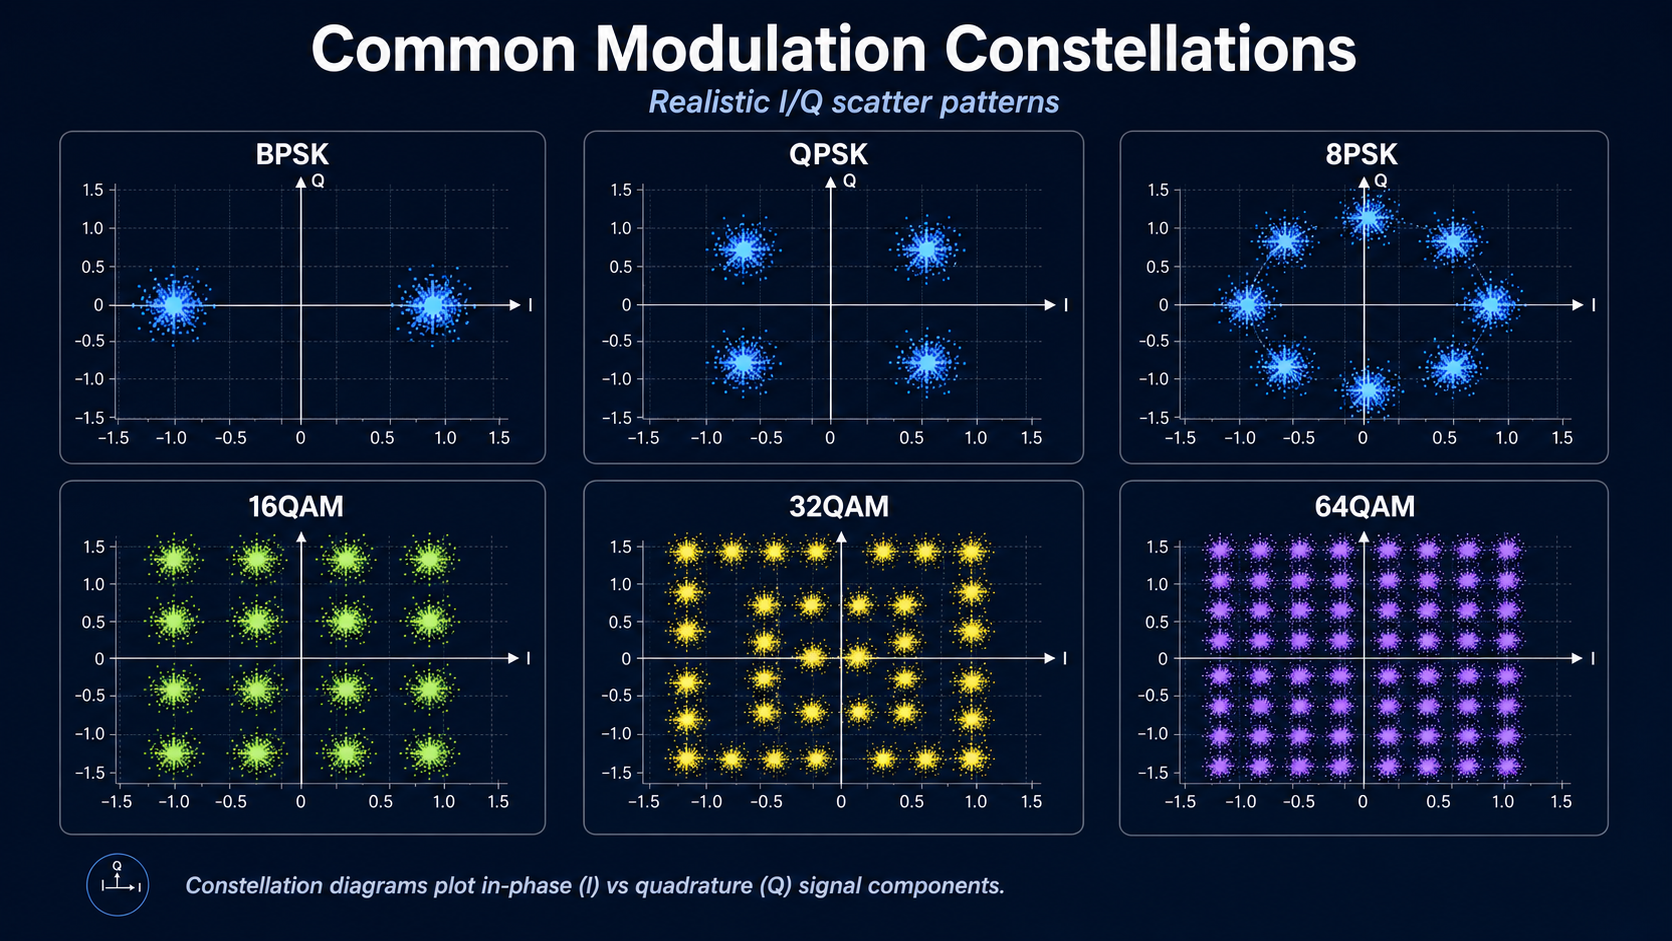
\includegraphics[scale=0.25]{../../KeyImages/constellation.png}

\newpage

\subsection{Feature Selection}

After training the feature-engineered model, I applied an information gain score to evaluate each engineered feature's relationship to modulation type prediction. The top 25 performing features were selected and used to train the final Random Forest model. This allowed me to test whether a smaller and more interpretable feature set could preserve most of the performance of the all-feature-engineered model.

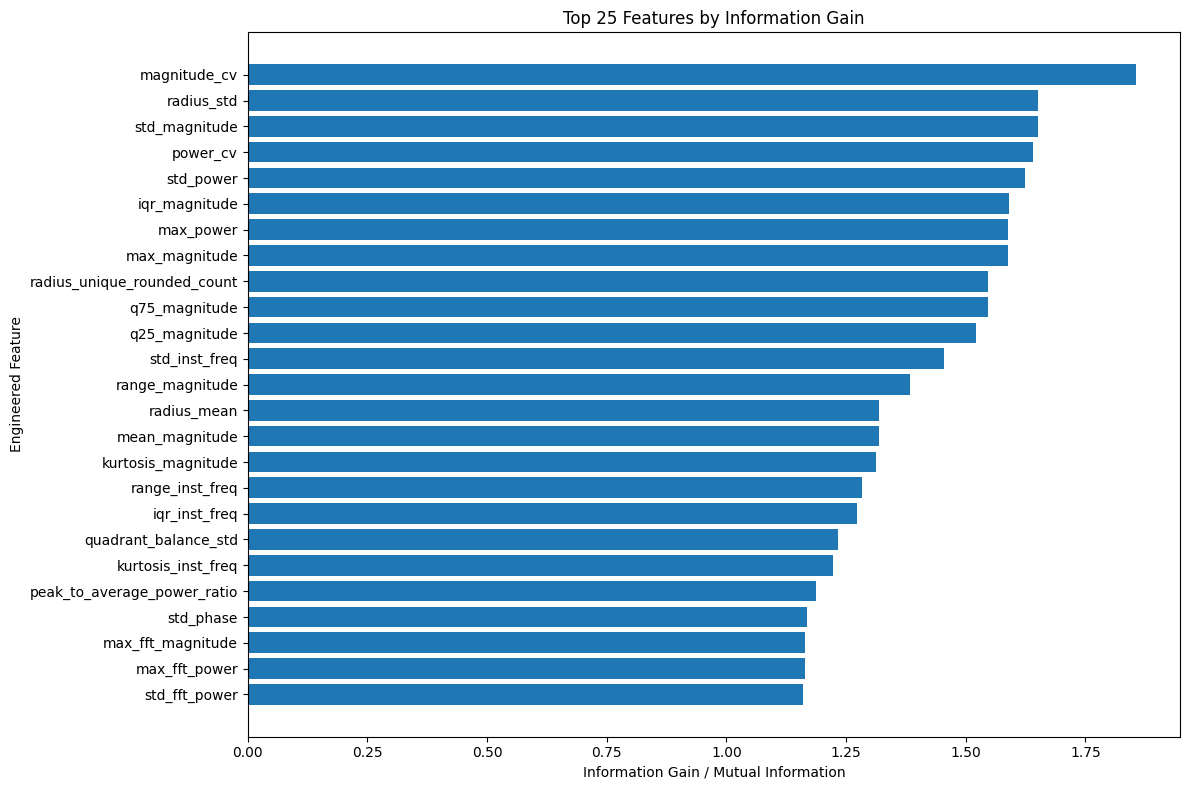
\includegraphics[scale=0.45]{../../KeyImages/top25Features.png}

\subsection{Simulation}

After model training and testing, I created a simulation to visually demonstrate the underlying concepts of the project. The textual simulation converts a string into bits and applies a simulated bit mask for modulation and optional encryption. It should be noted that the exact closeness of this bit masking and encryption process to a real RF receiver chain is not yet confirmed and requires further study. An audio example was also created where one audio output simulated a modulated and encrypted signal, while the other represented the correctly demodulated and decrypted signal.

\newpage

\section{Results}

The modeling results showed that the raw I/Q baseline was not enough by itself to make the Random Forest Classifier highly reliable for this 24-class modulation problem. The baseline model flattened each signal from its 1,024 I/Q timestamps into 2,048 raw input values. This model reached an accuracy of 36.21\% and a weighted one-vs-rest ROC-AUC of 0.8340. Since random guessing across 24 balanced modulation classes would be close to 4.17\% accuracy, this baseline was still learning useful structure from the I/Q values. However, it was not accurate enough to be considered strong for the objective of this project.

The feature-engineered model performed substantially better. After deriving math-based signal features, the all-feature-engineered RFC used 105 features instead of the 2,048 raw flattened I/Q values. This model reached 72.17\% accuracy, 71.20\% weighted precision, and 0.9780 weighted ROC-AUC. This was the best overall model and demonstrated that signal analyst-style transformations were more informative to the Random Forest than raw time-series values by themselves.

The selected-feature-engineered model tested whether most of the performance could be preserved with a smaller, more interpretable group of features. The top 25 features were selected using information gain, which reduced the feature-engineered set by 76.19\%. This model reached 69.38\% accuracy and 0.9729 weighted ROC-AUC. In practical terms, the selected-feature-engineered model lost about 2.79\% of accuracy and about 0.51\% of ROC-AUC compared to the all-feature-engineered model. Although the full engineered model remained the strongest, the top-25 model retained 96.13\% of the all-feature-engineered accuracy and 99.48\% of the all-feature-engineered ROC-AUC.

\begin{table}[H]
\centering
\caption{Random Forest model comparison on the highest-SNR reduced dataset.}
\label{tab:model-comparison}
\renewcommand{\arraystretch}{1.2}
\begin{tabularx}{\linewidth}{>{\raggedright\arraybackslash}p{2.25in}>{\raggedright\arraybackslash}X>{\centering\arraybackslash}p{0.75in}>{\centering\arraybackslash}p{0.85in}>{\centering\arraybackslash}p{0.95in}}
\toprule
\textbf{Model} & \textbf{Input / Feature Set} & \textbf{Features} & \textbf{Accuracy} & \textbf{Weighted ROC-AUC} \\
\midrule
Raw I/Q RFC Baseline & Flattened raw I/Q & 2,048 & 0.3621 & 0.8340 \\
All Engineered Features RFC & Engineered signal features & 105 & 0.7217 & 0.9780 \\
Top Selected Features RFC & Top information-gain features & 25 & 0.6938 & 0.9729 \\
\bottomrule
\end{tabularx}
\end{table}

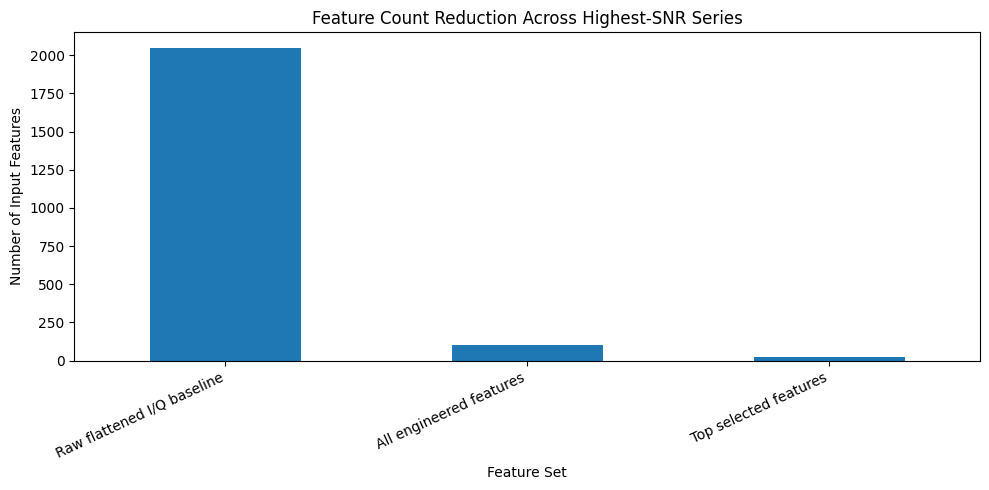
\includegraphics[scale=0.6]{../../KeyImages/modelFeaturesComparison.png}

Accuracy became the more useful metric in the report because the ROC-AUC values were already high for the engineered models and did not clearly explain the exact classification difference between them. ROC-AUC showed that the models generally ranked the correct modulation class well, but accuracy made the practical difference easier to explain: the all-feature-engineered model correctly predicted the modulation type more often than the selected-feature model, and both were much stronger than the raw I/Q baseline.

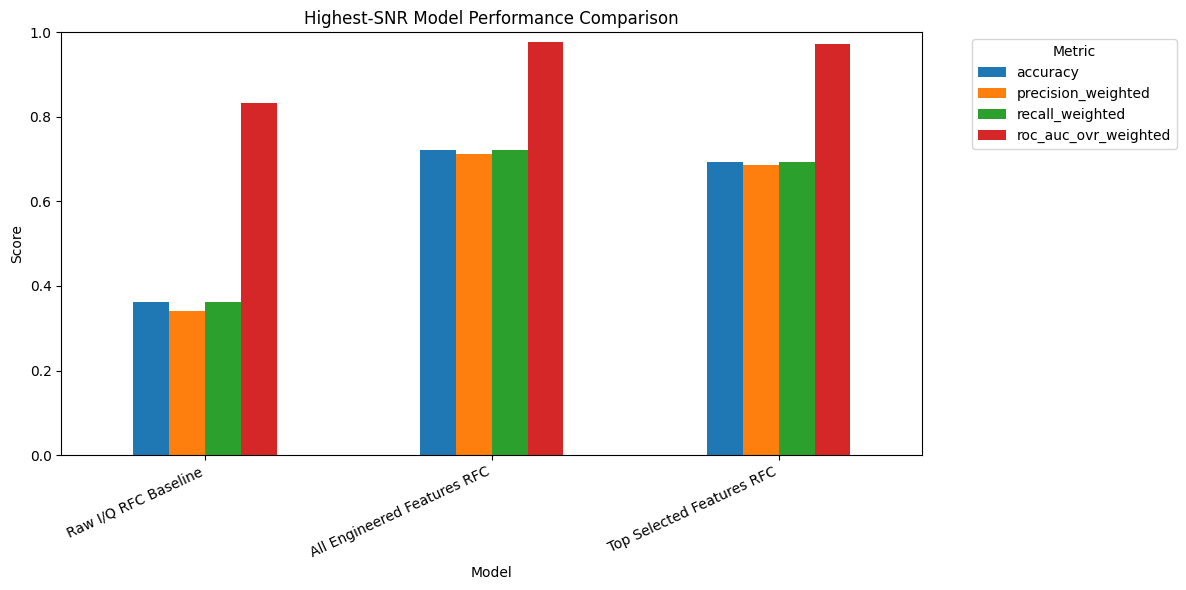
\includegraphics[scale=0.5]{../../KeyImages/modelMetricComparison.png}

\newpage

The simulation results were not evaluated as a formal machine learning metric because their purpose was different. The text and audio examples were conceptual demonstrations meant to make the invisible RF process easier to understand. The bit-string manipulation and intentionally distorted audio showed how information can become unreadable when the modulation or encryption assumptions are wrong, and how the same information becomes understandable when the correct process is applied. This was helpful for explaining why modulation detection and decryption are separate but connected steps in an RF hacking pipeline.

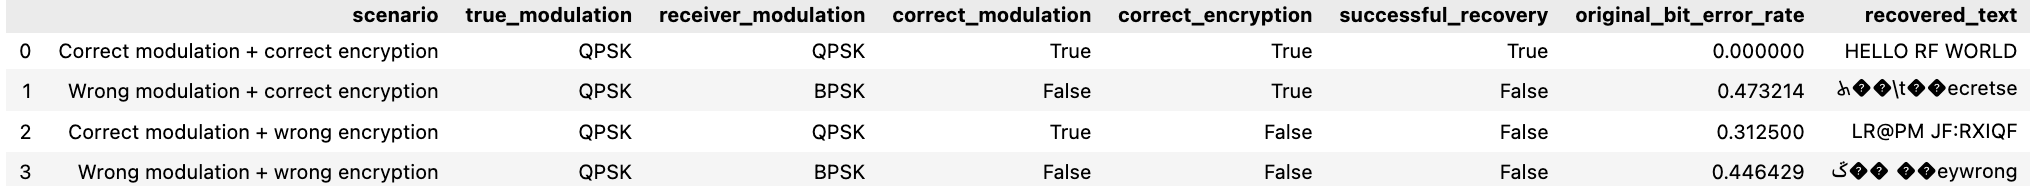
\includegraphics[scale=0.42]{../../KeyImages/bitSimulation.png}

\newpage

\section{Discussion}

The main interpretation of this project is that AI can help streamline parts of a signal analyst pipeline, but the model is only as good as the representation of the signal that it is given. The raw I/Q baseline proved that the model could learn something from direct waveform samples. However, the major jump in performance occurred when the signals were transformed into features that already carried more meaningful signal behavior. This supports the original reasoning that signal analysis is heavily mathematical and that coding those mathematical transformations can make the model's job easier.

This also helps explain why data quality mattered so much in the project. The original DeepSig dataset had over 2.5 million signals, but the proof-of-concept did not need to use all of them. By narrowing the data to the highest SNR value and selecting 1,000 examples from each modulation class, the model could first be tested under the clearest signal conditions. This was important because the project objective was not to solve every realistic RF problem immediately, but to determine whether the AI approach could work when the signal was relatively clean and the labels were reliable.

The selected-feature-engineered model was also important because it showed that the best model was not only a result of giving every possible feature to the classifier. Reducing 105 engineered features down to 25 selected features preserved most of the all-feature-engineered model's performance. This matters in a real pipeline because fewer features are easier to explain, faster to compute, and easier to evaluate when trying to understand why the model made a certain modulation prediction. Even though the all-feature-engineered model performed best overall, the selected-feature-engineered model was more compact and remained fairly close.

There are several important limitations to this project. First, the reduced dataset only used SNR = 30, which is the cleanest possible portion of the dataset. Real captured signals may include noise, distortion, interference, multipath issues, timing offsets, unknown sample rates, and frequency hopping. Second, the model only classified modulation type. It did not perform real demodulation, symbol timing recovery, carrier synchronization, or decryption. Third, the encryption and audio simulations were used for explanation and presentation rather than as proof that the code is equivalent to a real RF receiver chain. In other words, the simulation was useful for communication, but the machine learning portion was the stronger evidence for the project objective.

Another limitation is that a high ROC-AUC does not automatically mean a model is ready for real-world deployment. In this project, the high ROC-AUC values showed that the models could rank modulation classes well, but accuracy was more straightforward because the actual question was whether the model chose the correct modulation type. This is especially important in a multi-class problem, where a model can look strong under ROC-AUC while still making enough exact class mistakes to matter operationally.

\newpage

Overall, this project answered the objective partially but not completely. It demonstrated that an AI model can be trained to classify modulation types from recorded I/Q data, and that feature engineering based on signal analysis concepts significantly improves model performance. However, the project did not prove that an unknown real-time signal can be fully deciphered end-to-end. The next logical steps would be to train across multiple SNR levels, test against lower-quality signals, compare Random Forests against neural-network approaches, include more realistic receiver impairments, and eventually connect modulation detection to actual demodulation and cryptographic handling. In that respect, this project is best understood as a strong proof-of-concept for the modulation detection layer rather than a complete solution for deciphering any unknown signal.

\newpage

\section{Conclusion}

This project connected ethical hacking, RF signal analysis, and artificial intelligence by treating modulation detection as a layered security and signal-processing problem. The results showed that raw I/Q samples alone provided some useful information, but engineered signal features produced a much stronger Random Forest classifier. Feature selection further showed that a smaller group of top features could preserve most of the all-feature model's performance while improving interpretability.

The simulation reinforced the conceptual difference between modulation and encryption. Correct modulation helps recover the bitstream, while correct encryption handling is required to recover meaningful content. Together, the modeling and simulation support the idea that AI can assist in RF signal analysis, but only as part of a larger pipeline that must also address signal quality, timing, synchronization, demodulation, and cryptography.

\newpage

\section*{Resources Cited (IEEE)}
\addcontentsline{toc}{section}{Resources Cited}

\begin{enumerate}[label={\textbf{[\arabic*]}},leftmargin=0.55in]
    \item M. Lichtman, \textit{PySDR: A Guide to SDR and DSP Using Python}. Online textbook, 2024. [Online]. Available: \url{https://pysdr.org/}. [Accessed: May 9, 2026].
    \item T. J. O'Shea and N. West, ``Radio machine learning dataset generation with GNU Radio,'' in \textit{Proc. GNU Radio Conf. (GRCon)}, vol. 1, no. 1, 2016. [Online]. Available: \url{https://pubs.gnuradio.org/index.php/grcon/article/view/11}. [Accessed: May 9, 2026].
    \item T. J. O'Shea, J. Corgan, and T. C. Clancy, ``Convolutional radio modulation recognition networks,'' in \textit{Engineering Applications of Neural Networks}, pp. 213--226, Springer, 2016. [Online]. Available: \url{https://arxiv.org/abs/1602.04105}. [Accessed: May 9, 2026].
    \item T. F. Collins, R. Getz, D. Pu, and A. M. Wyglinski, \textit{Software-Defined Radio for Engineers}. Norwood, MA, USA: Artech House, 2018. [Online]. Available: \url{https://www.analog.com/en/resources/technical-books/software-defined-radio-for-engineers.html}. [Accessed: May 10, 2026].
    \item DeepSig Inc., ``RADIOML 2018.01A,'' \textit{DeepSig Datasets}, 2017. [Online]. Available: \url{https://www.deepsig.ai/datasets/}. [Accessed: May 13, 2026].
    \item J. G. Proakis, \textit{Digital Communications}, 4th ed. Boston, MA, USA: McGraw-Hill, 2001. [Online]. Available: \url{https://ocw.mit.edu/courses/6-451-principles-of-digital-communication-ii-spring-2005/pages/readings-and-lecture-notes/}. [Accessed: May 16, 2026].
    \item MathWorks, ``QPSK transmitter and receiver,'' \textit{MathWorks Documentation}. [Online]. Available: \url{https://www.mathworks.com/help/comm/ug/qpsk-transmitter-and-receiver.html}. [Accessed: May 17, 2026].
    \item GNU Radio, ``Guided tutorial PSK demodulation,'' \textit{GNU Radio Wiki}. [Online]. Available: \url{https://wiki.gnuradio.org/index.php?redirect=no&title=Guided_Tutorial_PSK_Demodulation}. [Accessed: May 17, 2026].
    \item GNU Radio, ``Simulation example: AM transmitter and receiver,'' \textit{GNU Radio Wiki}. [Online]. Available: \url{https://wiki.gnuradio.org/index.php/Simulation_example%3A_AM_transmitter_and_receiver}. [Accessed: May 17, 2026].
    \item National Institute of Standards and Technology, \textit{Advanced Encryption Standard (AES)}, FIPS PUB 197, Nov. 2001, updated May 2023. [Online]. Available: \url{https://nvlpubs.nist.gov/nistpubs/fips/nist.fips.197.pdf}. [Accessed: May 18, 2026].
    \item M. Dworkin, \textit{Recommendation for Block Cipher Modes of Operation: Methods and Techniques}, NIST Special Publication 800-38A, Dec. 2001. [Online]. Available: \url{https://nvlpubs.nist.gov/nistpubs/Legacy/SP/nistspecialpublication800-38a.pdf}. [Accessed: May 20, 2026].
    \item W. Diffie and M. E. Hellman, ``New directions in cryptography,'' \textit{IEEE Transactions on Information Theory}, vol. 22, no. 6, pp. 644--654, Nov. 1976, doi: 10.1109/TIT.1976.1055638. [Online]. Available: \url{https://www.scirp.org/reference/referencespapers?referenceid=1940218}. [Accessed: May 20, 2026].
\end{enumerate}

\end{document}
